\documentclass[conference]{IEEEtran}
%\documentclass[conference, final]{IEEEtran}


\usepackage[utf8]{inputenc}
\usepackage{cite}
\usepackage{amsmath}
\usepackage[acronym]{glossaries}
\usepackage{lipsum, adjustbox}

\usepackage{pgf}
\usepackage{tikz}
\usetikzlibrary{arrows}



\usepackage{algorithmic}
\usepackage{array}

\ifCLASSOPTIONcompsoc
  \usepackage[caption=false,font=normalsize,labelfont=sf,textfont=sf]{subfig}
\else
  \usepackage[caption=false,font=footnotesize]{subfig}
\fi

%\usepackage{fixltx2e}
%\usepackage{stfloats}
%\usepackage{dblfloatfix}
\usepackage{url}

\hyphenation{op-tical net-works semi-conduc-tor}


\usepackage[]{todonotes}
%\addbibresource{main.bib}

\begin{document}

\title{DNA : Une étude sur la Diversité logicielle et ses effets Négatifs sur l'Attaquant}

\author{
\IEEEauthorblockN{Philippe Troclet}
\IEEEauthorblockA{
%Email: 
philippe.troclet@polymtl.ca}
\and

\IEEEauthorblockN{Alexandre Mao}
\IEEEauthorblockA{
%Email: 
alexandre.mao@polymtl.ca}
\and
\IEEEauthorblockN{Paul Berthier}
\IEEEauthorblockA{
%Email: 
paul.berthier@polymtl.ca}
\and
\IEEEauthorblockN{Thomas Luinaud}
\IEEEauthorblockA{
%Email: 
thomas.luinaud@polymtl.ca}
}

\maketitle

\begin{abstract}

Bien que beaucoup aient mis en avant le risque posé par l'homogénéité au niveau logiciel, on ne sait pas précisément comment la diversité va réellement nuire à l'attaquant. Nous proposons d'apporter des éléments de réponse à l'impact de la diversité sur les attaques en fournissant deux modèles. L'un basé sur l'entropie qui nous permet de connaître le nombre moyen de machines infectées lors d'une attaque en fonction de la configuration logicielle du système, et prenant en compte le surcoût de cette diversité pour le défenseur. Dans le second, les différentes logiciels sont représentés et inter-connectés sous la forme d'un graphe, qui est ensuite parcouru par le \textit{malware.} Nous présentons enfin les résultats de la simulation de nos modèles sous différentes conditions, et montrons que la diversité logicielle permet bien de limiter les étendues des attaques.
\end{abstract} 
%\cite{ArchForCounter}

\IEEEpeerreviewmaketitle

\section{Introduction}
En janvier 2015, à la suite des attentats à Charlie Hebdo, une vague d'attaques a ciblé les sites des municipalités françaises.\cite{courrier}



%\lipsum[1]
%\hfill August 26, 2015

\section{Revue de littérature}
L'études des vulnérabilités au sein des logicielles n'est pas chose nouvelle. Des études quantitatives cherchant à modéliser le
nombre de failles de sécurités découvertes au cours du temps ont déjà été menées \cite{vulnerabilityDiscovery}. Et ce, avec des
résultats plus que satisfaisants. Il s'agissait dans cet article de parvenir à modéliser le taux de découvertes de vulnérabilités
afin de pouvoir l'anticiper et prévoir à l'avance de consacrer un certain nombre de personnes à la résolution des failles qui
serraient découvertes. Il s'agissait donc plutôt de mieux gérer ses effectifs. Une autre étude, plus centrée sur l'anticipation du
nombre de failles dans un programme, a vu le jour \cite{assessingVulnerabilities}. Cet article introduit également des modèles
permettant de caractériser le nombre de vulnérabilités que l'on trouvera si l'on consacre un certain "effort" à leur recherche.
%\lipsum[2]


\section{Hypothèses et Méthodologie}
Afin de réaliser notre analyse, nous avons procédé en deux étapes.
Tout d'abord nous avons défini un modèle mathématique permettant d'estimer le coût d'une attaque et de la défense.
Puis nous avons appliqué notre modèle en analysant des jeux de données.
Dans cette section, nous expliquerons tout d'abord notre modèle mathématiques puis nous expliquerons comment nous avons appliqué ce modèle à nos données.
%grandeur concernant la biodiversité du système.

\subsection{Modèle mathématique}\label{sec:modelMath}

Afin de définir notre modèle mathématique, nous avons basé notre approche sur un phénomène physique homologue : la thermodynamique.
Nous allons donc définir une entropie logicielle qui sera liée à l'hétérogénéité du système.
Redéfinissons tout d'abord le premier principe de la thermodynamique~: Il y a conservation de l'énergie. 

\[
\Delta E = \Delta U = W + Q
\]

$\Delta E$ est la variation d'énergie du système, $\Delta U$ est la variation d'énergie interne du système, $W$ est le travail reçu par le système et $Q$ est la chaleur reçue par le système.

La seconde loi de la thermodynamique nous donne :
\[
S_{creation} = \Delta S_{syst} + \Delta S_{ext} \geq 0
\]

Cela se caractérise dans notre cas par un principe simple~: tout changement de configuration dans notre système, quel qu'il soit, crée de l'entropie et donc augmente, au moins temporairement, la difficulté de l'attaque.
Dans le cas ou l'entropie de notre système diminuerai, il y a tout de même une augmentation de l'entropie du côté de l'attaquant. Cela s'explique par le fait que l'état du nouveau système lui est inconnu. Il doit à nouveau refaire toute son analyse avant d'effectuer une nouvelle attaque. On notera également que sans action spécifique du défenseur, en laissant les administrateurs des sous-systèmes faire les mises à jour indépendamment, l'entropie du système global va augmenter de manière naturelle au cours du temps. 

Le second principe peut également s'écrire :

\[
\frac{Q}{T} \leq \Delta S_{syst}
\]

À quoi correspondent toutes ces grandeurs physiques dans notre système ? On va associer Q à l'effort fourni pour effectuer des mises à jours (Si Q est nul, il n'y a pas d'entropie créée), et W sera le travail fourni par l'attaquant pour effectuer son attaque. Du côté du défenseur, Q va en réalité être négatif. En effet, on va associer l'énergie du système à la quantité d'attaques subies. On veut donc en permanence le "refroidir".
De même, la température T va être associée à la vulnérabilité des versions des logiciels du système. Plus les versions sont anciennes, plus elles seront vulnérables et donc la température va augmenter en fonction du temps.
On notera également que plus l'entropie du système est grande, plus le travail à fournir par l'attaquant sera important.



\subsection{Application du modèle}
Dans cette section, nous expliquons comment nous avons appliqué notre modèle mathématiques.
Nous avons dans un premier temps récupérer les données des différentes versions de serveur Web utilisés par les communes françaises ainsi que des vulnérabilités associées.
Finalement nous avons recoupé les différentes information et effectué le calcul mathématiques.

\subsubsection{Récupération des données}
Pour faire une études comparative, nous avons récupéré un jeu de donnée sur les serveurs web utilisés par les communes françaises datant de mars 2015.
Par la suite, nous avons généré un jeu de donnée à partir du même script afin de connaître l'état actuel des systèmes.
Finalement nous avons récupéré les différentes failles de sécurité connu pour les différentes version de ces logiciels.

Les différentes failles de sécurité ont été récupéré depuis~\cite{vulnDatabase}

Une fois les données trouvée, nous avons réalisé un recoupement des données.
Pour cela, nous avons considéré que les versions de logiciel donnés par les serveurs sont les versions réellement utilisés et également que les serveur n'envoyant pas d'informations sont sécurisé de base.


\subsubsection{Application du modèle mathématique}
Notre modèle mathématique prend en compte d'une part la variabilité des différents systèmes dans l'environnement ainsi que les mises à jours.
En effet, nous avons précédemment expliqué qu'une mise à jours amenait un travail supplémentaire à fournir par l'attaquant.
Nous appliquons donc simulation, une où l'on considère la complexité de l'attaque liée à l'hétérogénéité du système et une où l'on considère l'impact des mises à jours sur l'entropie.

\paragraph{L'impact de l'hétérogénéité du système}
Le fait d'avoir un système hétérogène amène à une augmentation du nombre total de vulnérabilité.
Cependant cette diversité peut rend une attaque global plus complexe vue que chacun des systèmes sera sensible à des attaques différentes.
La figure~\ref{fig:heteImpactVuln} exprime cette notion de non concordance entre les vulnérabilités et leur version.
Dans cette figure, les nœuds "Ln" représentent une version de logiciel et les noeuds "Vn" représentent un numéro de vulnérabilité.
Nous voyons que certaine version n'ont aucune vulnérabilité communes avec d'autre tel que "L4" avec et "L5".
Dans ce cas, il est plus compliqué d'attaquer les deux système simultanément.
Cependant, si nous prenons le cas de "L1" et "L2", ils sont tout deux sensibles à "V1" et "V2".
Dans ce cas, la diversité amène une augmentation du risque d'attaques.


\begin{figure}
\centering
%peut être la faire avec des exemple de vulnérabilité réelles
\begin{tikzpicture}[->,>=stealth',shorten >=1pt,auto,node distance=1cm,
  thick,version node/.style={circle,fill=blue!15,draw,
  font=\sffamily\small\bfseries,minimum size=5mm}, vulne node/.style={circle,fill=red!15,draw,
  font=\sffamily\small\bfseries,minimum size=5mm}]
  
  \node[version node] (L0) {L1};
  \node[version node] (L1) [below of=L0] {L2};
  \node[version node] (L2) [below of=L1] {L3};
  \node[version node] (L3) [below of=L2] {L4};
  \node[version node] (L4) [below of=L3] {L5};
  
  \node[vulne node] (V1) [right of=L0, node distance=3cm] {V1};
  \node[vulne node] (V2) [below of=V1] {V2};
  \node[vulne node] (V3) [below of=V2] {V3};
  \node[vulne node] (V4) [below of=V3] {V4};
  \node[vulne node] (V5) [below of=V4] {V5};

%connexion vulnerabilité 1
  \draw [-latex'] (V1) -- (L0);
  \draw [-latex'] (V1) -- (L1);
  \draw [-latex'] (V1) -- (L2);
  \draw [-latex'] (V1) -- (L4);
  
%connexion vulnerabilité 2
  \draw [-latex'] (V2) -- (L0);
  \draw [-latex'] (V2) -- (L1);
  \draw [-latex'] (V2) -- (L2);

%connexion vulnerabilité 3
  \draw [-latex'] (V3) -- (L0);
  \draw [-latex'] (V3) -- (L2);

%connexion vulnerabilité 4
%  \draw [-latex'] (V4) -- (L4);
  \draw [-latex'] (V4) -- (L2);
  \draw [-latex'] (V4) -- (L3);

%connexion vulnerabilité 5
  \draw [-latex'] (V5) -- (L4);
 
  
\end{tikzpicture}
\caption{Schéma de la relation entre la version d'un logiciel et les vulnérabilités associées.}
\label{fig:heteImpactVuln}
\end{figure}

\paragraph{L'impact des mises à jours}
Dans le paragraphe précédent, nous avons expliqué l'intérêt qu'il y a à la diversité des versions.
Toutefois, nous n'avons pas pris en compte l'ancienneté d'une vulnérabilité. 
L'ancienneté d'une vulnérabilité la rend plus facilement exploitable car plus connu.
De plus, comme expliqué dans la section~\ref{sec:modelMath}, le fait de faire des mises à jours forcera l'attaquant à augmenter l'effort pour être capable de s'adapter à ce changement.

\section{Modélisation}
\subsection{Modèle mathématique}\label{sec:modelMath}

Notre objectif est de déterminer le nombre moyen de machines infectées lors d'une attaque, en fonction de la configuration logicielle du système. En effet, on peut considérer que dans un système à grande échelle, avec un certain degré de redondance, une attaque n'est concluante que si un certain pourcentage des machines a été infecté. Il peut donc être plus intéressant d'optimiser le nombre moyen de machines infectées par attaque plutôt que la probabilité d'infection (c'est à dire préférer une probabilité d'infection plus importante, mais avec un faible nombre de machines infectées à chaque attaque plutôt qu'une probabilité d'infection plus faible, mais où une très grande partie du système serait affecté en cas d'attaque).\\
Pour cela, nous allons définir "l'entropie" du système. Cette grandeur vient à l'origine de la thermodynamique et caractérise le "désordre" d'un système. Claude Shannon a eu l'idée de transposer cette grandeur au domaine de la théorie de l'information\cite{entropie_shannon}.\\
Dans notre cas, nous allons reprendre sa formulation, et allons définir l'entropie de notre système comme son degré d'hétérogénéité, c'est à dire la variété des logiciels qui y sont installés pour une application donnée.
Pour cela, définissons $E_v$ comme l'ensemble des logiciels installés sur notre système de $n$ machines pour l'application fixée (e.g. un serveur web). Pour chaque élément de l'ensemble, posons $p_i$ la probabilité que ce logiciel se retrouve installé sur l'une des machines. 
On a donc:

\[
\sum_{E}p_i=1
\]

On pose alors H l'entropie de Shannon :

\[
H=-\sum_E p_i \log(p_i)
\]

On pose également $T$ comme l'ancienneté moyenne des logiciels de notre système, chaque logiciel ayant une ancienneté $T_i$ (on définit l'ancienneté d'un logiciel comme le temps écoulé depuis sa publication)  :

\[
T=\sum_E p_i T_i
\]

On recherche alors le nombre moyen d'infections par attaque en fonction de l'entropie et de l'ancienneté moyenne de notre système. Comme un \textit{malware} ne peut cibler qu'un unique logiciel, plus notre système sera hétérogène, moins le \textit{malware} pourra se propager. En revanche, plus les versions des logiciel seront anciennes, plus le nombre de failles qui y auront été découvertes sera importante, et donc plus la probabilité d'infection initiale sera importante. Il est donc important de prendre en compte ces deux paramètres de notre système pour calculer l'importance d'une infection potentielle que l'on pose : 

\[
N_{infection} = f(H,T) = P_{attaque}(T)*D(H)
\]

En ce qui concerne la probabilité de l'infection initiale, nous considérerons par la suite qu'elle croît exponentiellement avec l'ancienneté moyenne de notre système. Nous la définissons donc comme suit :

\[
P_{attaque}(T) =1- \exp^{-\lambda*T}
\]

Si $T=0$, le logiciel vient de sortir. Comme toutes les failles connues sont corrigées, et qu'il n'y a pas de failles \textit{zero day}, la probabilité d'infection est nulle. Au contraire, plus $T$ augmente, plus le nombre de failles découvertes et leur diffusion augmentent, et la probabilité d'infection tend vers 1. $\lambda$ est un paramètre qui sert à ajuster la vitesse à laquelle la probabilité d'infection augmente avec l'ancienneté du logiciel.\\

On définit $H_{un}$ comme l'entropie pour une distribution uniforme avec n logiciels différents (chaque ordinateur a un logiciel différent) :

\[
H_{un} = -\sum_n \frac{1}{n} * \log(\frac{1}{n}) = \sum_n \frac{\log(n)}{n} = \log(n)
\]

Il reste à établir la formule reliant l'entropie et la diffusion de l'infection. Dans un premier temps, nous allons établir le mode le plus simple possible : un modèle linéaire en H. En cas d'infection, on considère que k machines sont touchées en moyenne, sur un total de m. On a alors :

\[
k=1+(m-1)*(1-\frac{H}{H_{un}}) =m-\frac{m-1}{\log(n)}*H
\]

Ce premier modèle est cohérent en $H=0$, puisqu'on est alors en présence d'un système avec un unique logiciel. En cas d'infection, $k=n$ : toutes les machines sont touchées puisqu'il n'y a pas de diversité logicielle (le \textit{malware} peut se propager partout).\\
Il est aussi cohérent pour $H=H_{un}$. En effet, chaque machine a alors un logiciel différent, et alors $k=1$ : seulement la première machine est infectée, le \textit{malware} n'arrive pas du tout à se propager.\\
La formule finale est donc :


\[
N_{infection}=[1-\exp^{-\lambda_1*T}] * [m-\frac{m-1}{\log(n)}*H]
\]

On peut remarquer que d'après notre modèle, la meilleure façon de ne pas se faire affecter est d'installer la même dernière version du logiciel sur toutes les machines, ou encore afin de ne pas propager l'infection dans le système, d'installer des logiciels différents sur chaque machine. Cela parait assez intuitif, et on peut se dire au premier abord qu'il suffit donc de se placer dans l'une ou l'autre de ces situations. Cependant, il ne faut pas oublier qu'en pratique, il est presque impossible dans un système de taille importante et en production de maintenir en permanence les logiciels à jour. De plus cela implique des coûts importants. De même, une trop grande diversité des logiciels implique un coût de maintenance élevé, puisqu'il faut préparer des procédures de mise à jour différentes pour chacun d'entre eux.
Ainsi, afin de rendre notre modèle plus réaliste, nous allons y introduire ces coûts. Il ne suffira plus alors de minimiser le taux de pénétration du \textit{malware} dans notre système, mais plutôt ce taux \textbf{plus} le coût correspondant à la maintenance du système.

Nous posons donc $C_T$ le coût de maintenance par unité de temps selon l'ancienneté moyenne des logiciels que l'on vise à avoir :

\[
C_T=m*\frac{1}{T}
\]

Ce coût est linéaire en $\frac{1}{T}$, puisque si nous voulons avoir une ancienneté moyenne des logiciels deux fois plus petite, il faudra logiquement effectuer les mises à jour deux fois plus régulièrement.

Nous posons également $C_H$ le coût de maintenance par unité de temps qui sera lui fonction de l'entropie de notre système et du nombre de logiciels qui y sont installées :

\[
C_H = g(n,H)
\]

$C_H$ dépend du nombre de logiciels dans notre système, comme expliqué précédemment, mais il dépend également de l'entropie, car si il y a uniquement une machine équipée d'une version donnée d'un logiciel, alors il suffira d'y faire une mise à jour manuelle, alors que si cette version est plus répandue, il faudra alors préparer une procédure de mise à jour automatique. Cependant,cette fonction de coût est très difficile à définir, et dépendra fortement des procédures en place dans chaque département IT. C'est pourquoi nous ne donnons pas sa forme.

Nous pouvons alors poser le coût total pour le défenseur:

\[
C_{Total}=k_1*N_{infection}+k_2*C_T+k_3*C_H
\]

Les coefficients $k_1$, $k_2$ et $k_3$ sont à définir par l'administrateur du système afin que les résultats collent à ses exigences spécifiques en terme de diffusion du \textit{malware} par rapport à ses propres coûts de maintenance informatique.

\begin{figure}[!ht]
\centering
     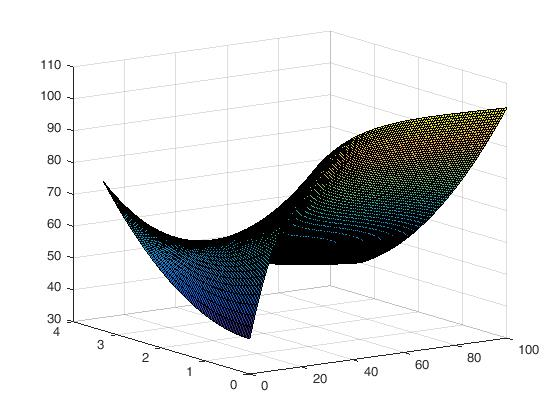
\includegraphics[width=1.0\linewidth]{Paul/Matlab/3D.jpg}
     \caption{Modélisation avec Matlab}
     \label{matlab}
\end{figure}

\begin{figure}[!ht]
\centering
     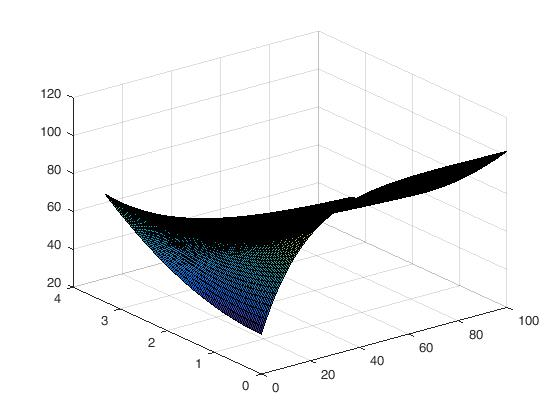
\includegraphics[width=1.0\linewidth]{Paul/Matlab/3D_proj.jpg}
     \caption{Projection de la modélisation avec Matlab}
     \label{matlab_proj}
\end{figure}

Sur les figures \ref{matlab} et \ref{matlab_proj}, on observe une simulation de notre modèle sous Matlab. Les paramètres ont été choisis de façon arbitraire, et donc les valeurs numériques ne sont pas significatives. Cependant, on observe dans le cas présenté un minimum local, qui correspond au compromis idéal entre coût lié à  l'ancienneté moyenne des versions et à leur entropie et coût lié à la diffusion dún \textit{malware}. Cela confirme donc qu'un défenseur pourra se servir de ce modèle pour, connaissant les paramètres propres à son système, agir de façon adéquate sur sa diversité logicielle.

\begin{figure}[!ht]
\centering
     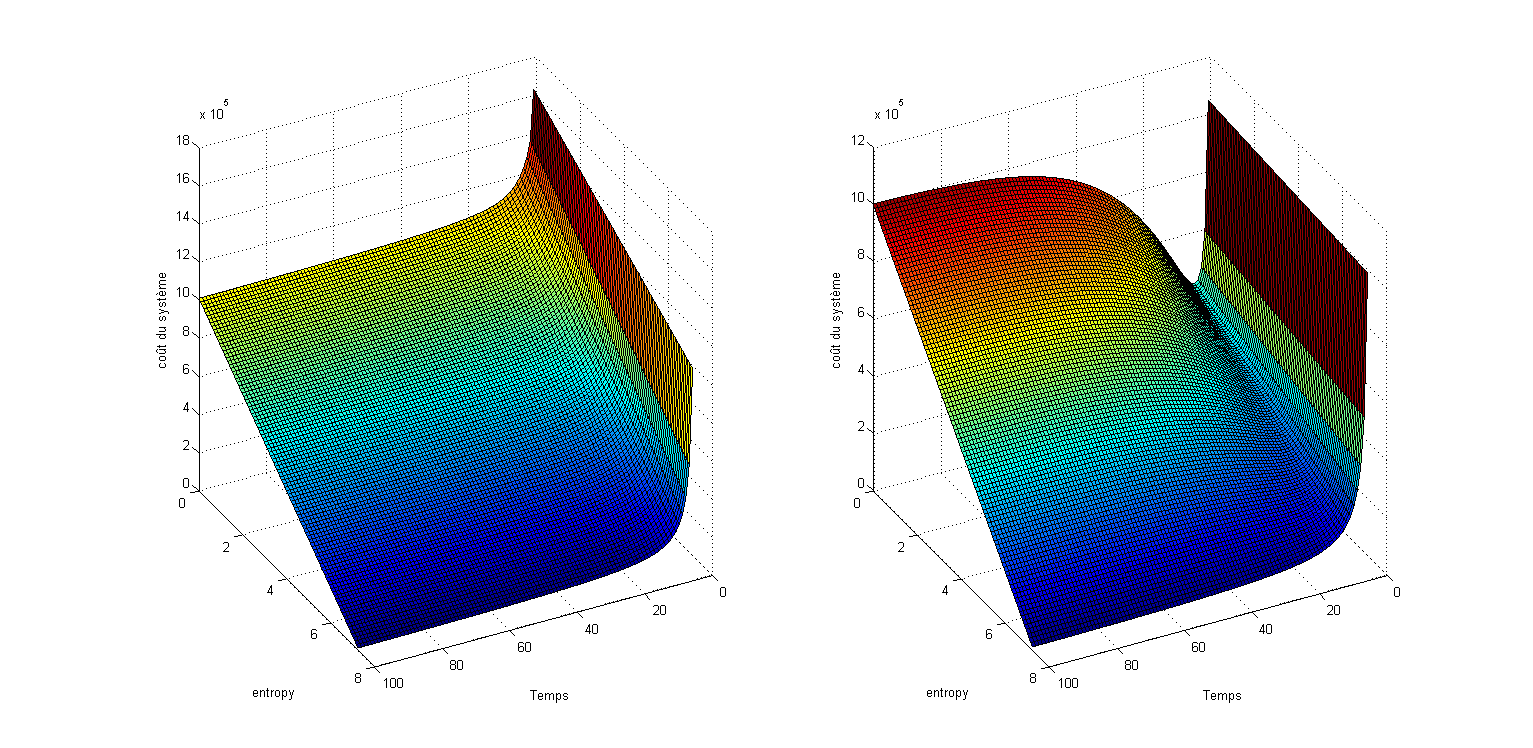
\includegraphics[width=1.0\linewidth]{Paul/Matlab/lambda_var.png}
     \caption{Impact de la variation de lambda (gauche=1, droite=0.05)}
     \label{lambda}
\end{figure}

Sur la figure \ref{lambda}, on observe l'influence de la vitesse de découverte des vulnérabilités $\lambda$. On y voit que, peu importe $\lambda$ (le seul paramètre sur lequel peut influence l'attaquant en accentuant sa recherche de vulnérabilités), le défenseur gagne à augmenter l'entropie de son système. C'est là la grande force de ce moyen de défense : l'attaquant n'a pas vraiment de moyen de le contourner.


\section{Simulation}
Pour valider notre modèle, nous avons développé une simulation basée sur un graphe.
Chaque machine de notre système y est représentée par un nœud, et possède en moyenne \textit{l} liaisons vers d'autres machines

\begin{figure}[ht]
\centering
     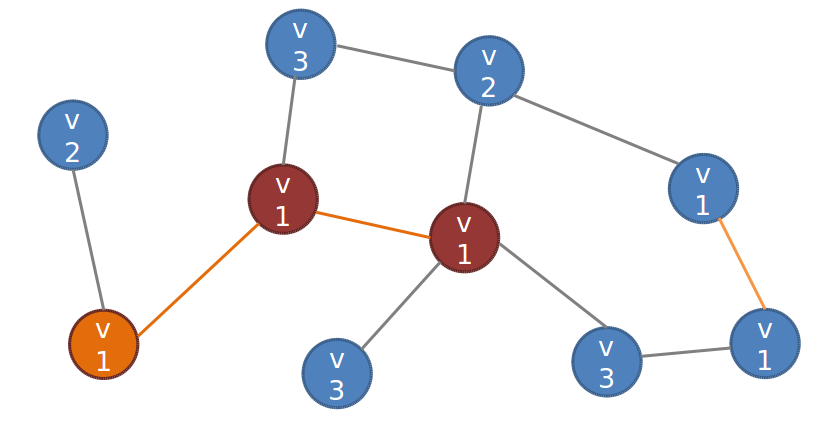
\includegraphics[width=1.0\linewidth]{Paul/python/graph.png}
     \caption{Représentation du système par un graphe}
     \label{normal_case}
\end{figure}

La première étape est de définir la répartition des versions dans le système. Afin de faire varier l'entropie, on utilise une distribution de Dirichlet.

\begin{figure}[ht]
\centering
     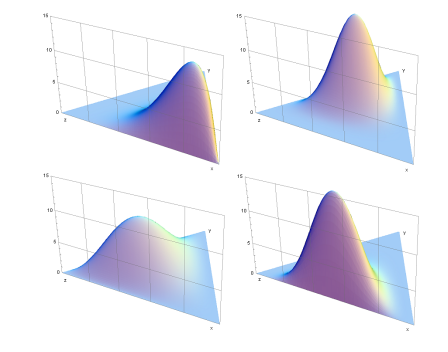
\includegraphics[width=1.0\linewidth]{Paul/dirichlet.png}
     \caption{Distribution de Dirichlet (source: Wikipedia)}
     \label{normal_case}
\end{figure}


\section{Discussion et travail ultérieur}
Nous avons proposé dans cet article un modèle sur le taux d'infection en fonction de la diversité logicielle. Ce modèle bien
qu'intéressant comporte quelques limitations sur lesquelles une recherche ultérieure serait souhaitable. En premier lieu nous avons
considéré qu'un attaquant serait plus apte à maximiser le nombre d'infections plutôt que la probabilité d'infecter une machine.
Cette hypothèse est raisonnable dans de nombreuses situations mais elle peut sembler inappropriée dans certains cas. En effet, si
l'attaquant
cherche à récupérer des informations confidentielles mais a priori présentes sur un petit nombre d'ordinateurs au sein d'une
compagnie, il sera alors plus intéressant pour lui de maximiser la probabilité d'infecter ces machines et non le nombre total de machines infectées.
\newline

Un autre point important pour compléter nos résultats est la détermination de constantes. Nous avons présenté un
modèle de coût, qui étudier de manière plus approfondie pourrait avoir de nombreuses applications. En particulier, il permettrait de chiffrer un
coût lors d'un audit et de donner des métriques tangibles qui pourraient servir de base pour déterminer un plan
d'action. Une telle recherche nécessiterait des compétences économiques pour évaluer les différents coûts mais aussi un
savoir-faire technique pour déterminer la dangerosité d'un système.
\newline

Nos équations se basent sur une constante $\lambda$ dont la valeur doit être déterminer afin d'obtenir des résultats numériques. Une
études de champs est souhaitable pour approximer le $\lambda$ moyen d'une attaque. Il serait également intéressant de déterminer un
$\lambda$ pour différents types d'attaques auxquels nous pouvons être confrontés.
\newline

Nos résultats se basent sur l'hypothèse qu'un malware ne peut exploiter qu'une vulnérabilité et que cette vulnérabilité
ne peut affecter deux logiciels distincts. Nous aurions pu prendre en compte plutôt une vulnérabilité qu’une version de logiciel comme cela a été fait par  Neti et al.\cite{softwareDiversity:Security}
 Il serait intéressant de voir l'impact de ce hypothèse notre modèle.

Enfin, nous pourrions d'un travail futur de confronter nos résultats à des situations concrètes via une étude de mesures issues de
données réelles. Il est important de vérifier les résultats des simulations en les mettant en corrélation à des données tirées de systèmes réels. 
\newline

Bien qu'ayant ses limites, nos résultats restent valables dans les hypothèses annoncées. Ces dernières correspondent
qu'à certaines situations possibles et sont valables dans ces cas-là. Et, les simulations confirment la relation
linéaire entre l'entropie et le nombre d'infections. 


\section{Conclusion}
Le modèle présenté ici, est, à notre connaissance, le seul modèle permettant de mesurer le nombre d'infection en fonction de la
diversité de de l'ancienneté du système. Bien qu'un travail en amont soit nécessaire, les premiers résultats sont encourageants. 
\newline

En effet, nos expérimentations montrent, d'une part l'existence d'un lien entre l'entropie et le nombre de machines infectées et d'autre part que l'hypothèse d'une
relation linéaire entre ces quantités est raisonnable. \`A l'heure actuelle, le nombre d'applications ayant suffisamment de
déclinaisons pour que l'entropie d'un système puisse être supérieure à deux est en effet très faible. De ce fait, nos résultats
peuvent s'appliquer à de nombreux cas dans la vie réelle. 
\newline

Nous avons de plus présenté un modèle de coût, qui, une fois les constantes déterminées et une fonction d'évaluation du coût de
maintenance correctement définie, permettra de guider un administrateur réseau dans ses choix pour la maintenance de la
plateforme à sa charge.
\newline

Nous allons clôturer cet article, par le principe suivant: la diversité favorise la sécurité.



\bibliographystyle{IEEEtran}
\bibliography{paper1} % IEEEabrv, 
%\printbibliography
\end{document}
